\subsection{Function Shape}

\begin{figure}
	\centering
	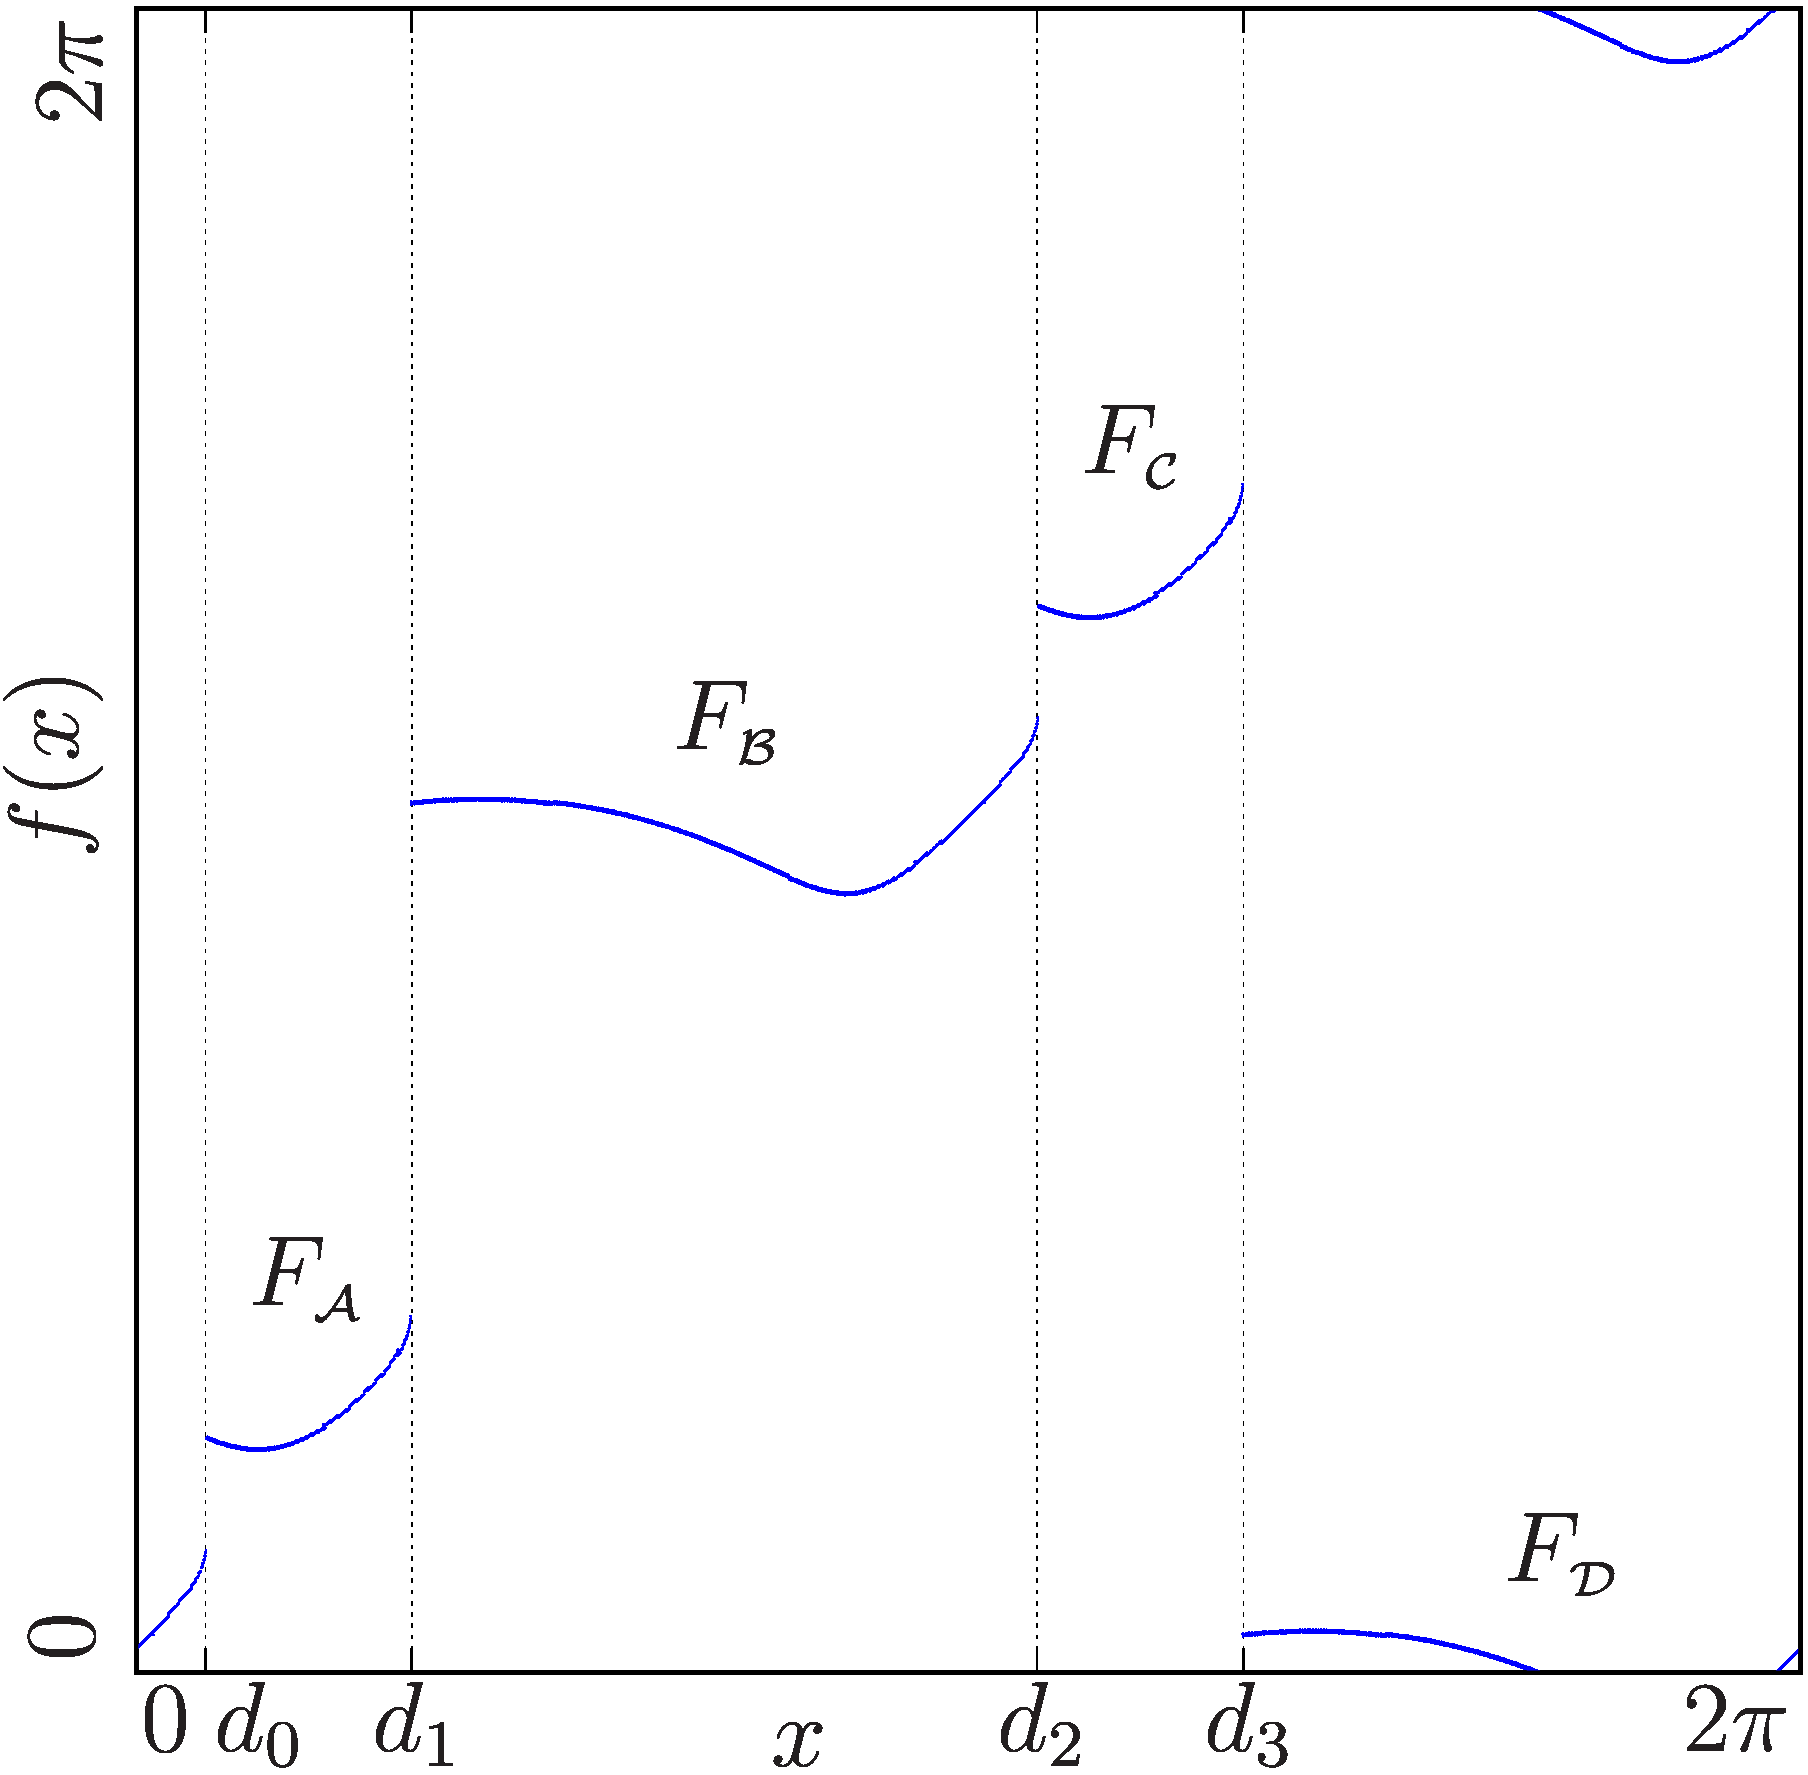
\includegraphics[width=.5 \textwidth]{../Figures/5/5.1/illustration.png}
	\caption[The shape of the original model function]{
		The shape of the original model function with the parameter values $E_0 = 15$ and $\chi_0 = 0.2$.
	}
	\label{fig:setup.char.shape}
\end{figure}

This section is concerned with the overall shape and number of branches of the original model function.

\Cref{fig:setup.char.shape} shows the shape of the original model function.
One can immediately see that the model function has 4 branches.
This is also evident from the model definition given in \Cref{sec:state.og.def}.
Also, we know from \Cref{sec:state.og.dynamics} that the model has the symmetry described by \Cref{equ:state.og.sym}.
So the branches $F_\A$ and $F_\C$ are identical.
The same is true for the branches $F_\B$ and $F_\D$.

There are no fixed points in the parameter regions that this thesis is concerned with.
That means, the function is always larger than the bisector $y=x$.
Also, for the most part the slope of the function is not steep.
Meaning that the absolute value of the model functions derivative is below $1$ for a majority of the state space.
A model where the absolute value of the derivative of its model function is below $1$ for the whole state space is called contractive.
In such a model, every fixed point and cycle is stable.
